\section{Results} 
\subsection{Optimal \(\epsilon\) selection}
The data is expected to be positively skewed
so the medians were found in order to compare the performance.
Figure \ref{fig:bidir_correlated} shows the distance \(d_J\) of the trials
for bidirectional RRT for different values of \(\epsilon\), with the median highlighted.
The corresponding plot for the
balanced bidirectional RRT is shown in figure \ref{fig:balanced_correlated}.

The Spearman's Rank Correlation test,
with the null-hypothesis that \(d_J\) is uncorrelated with \(\epsilon\),
gave a p-value of \(1\cdot 10^{-19}\) for the bidirectional RRT,
and a p-value of \(6\cdot 10^{-21}\) for the balanced bidirectional RRT.
This implies that \(d_J\) and \(\epsilon\) are correlated in both algorithms.
\(H_{0,corr}\) is rejected.

To give each algorithm the best chance of providing the optimal path,
the optimal \(\epsilon\) was found for both algorithms.
The optimal \(\epsilon\) was found by taking the lowest median.
For bidirectional RRT, \(\epsilon_{bi}\) was found to be \(2.25\) jointspace units,
and for balanced bidirectional RRT it was found to be \(2.15\) jointspace units.

\begin{figure}[h]
 \centering
 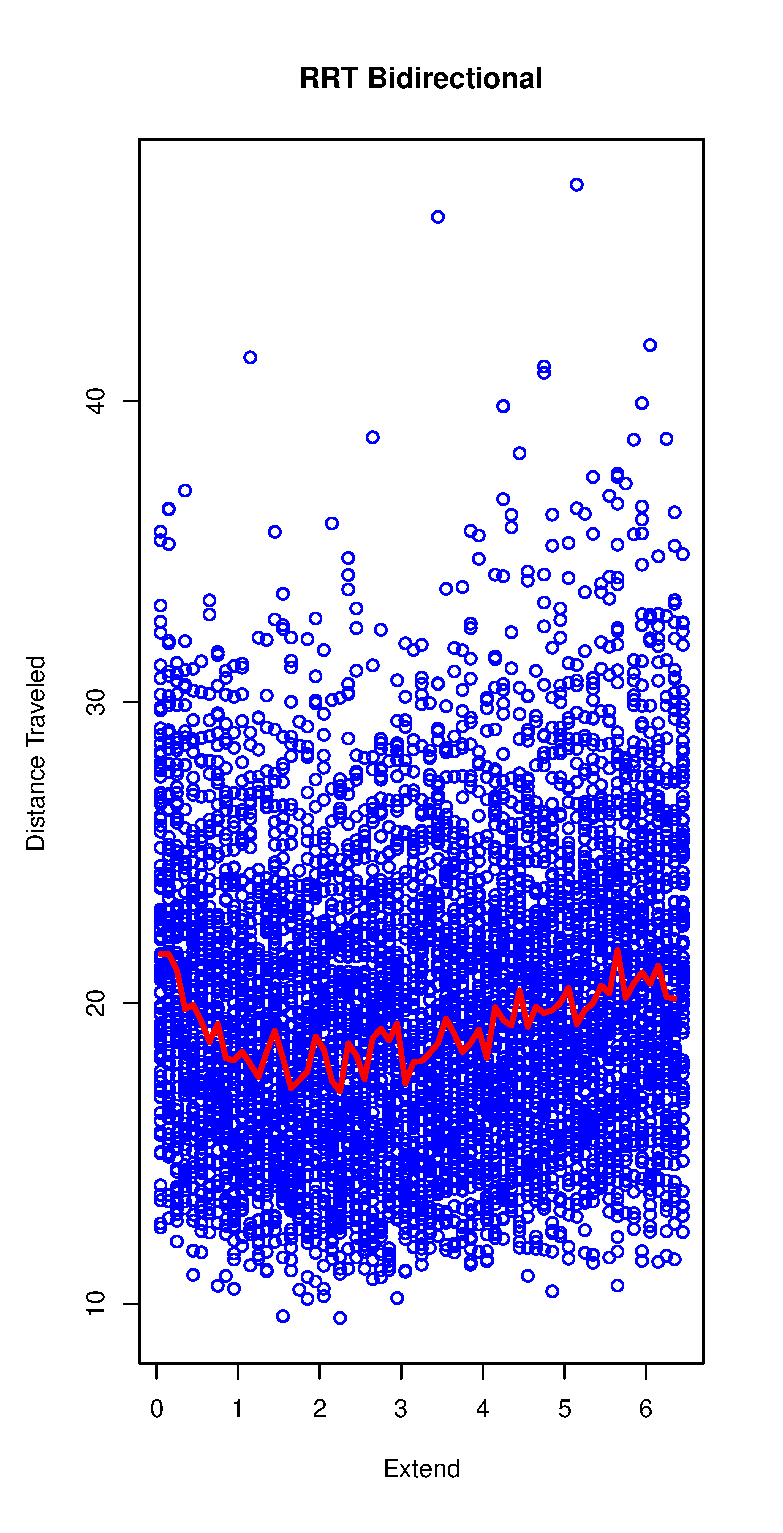
\includegraphics[width=\figsize]{graphics/bidirectional_correlation}
 \caption{\(d_J\) of the bidirectional RRT planner (blue) with median highlighted (red).}
 \label{fig:bidir_correlated}
\end{figure}

\begin{figure}[h]
 \centering
 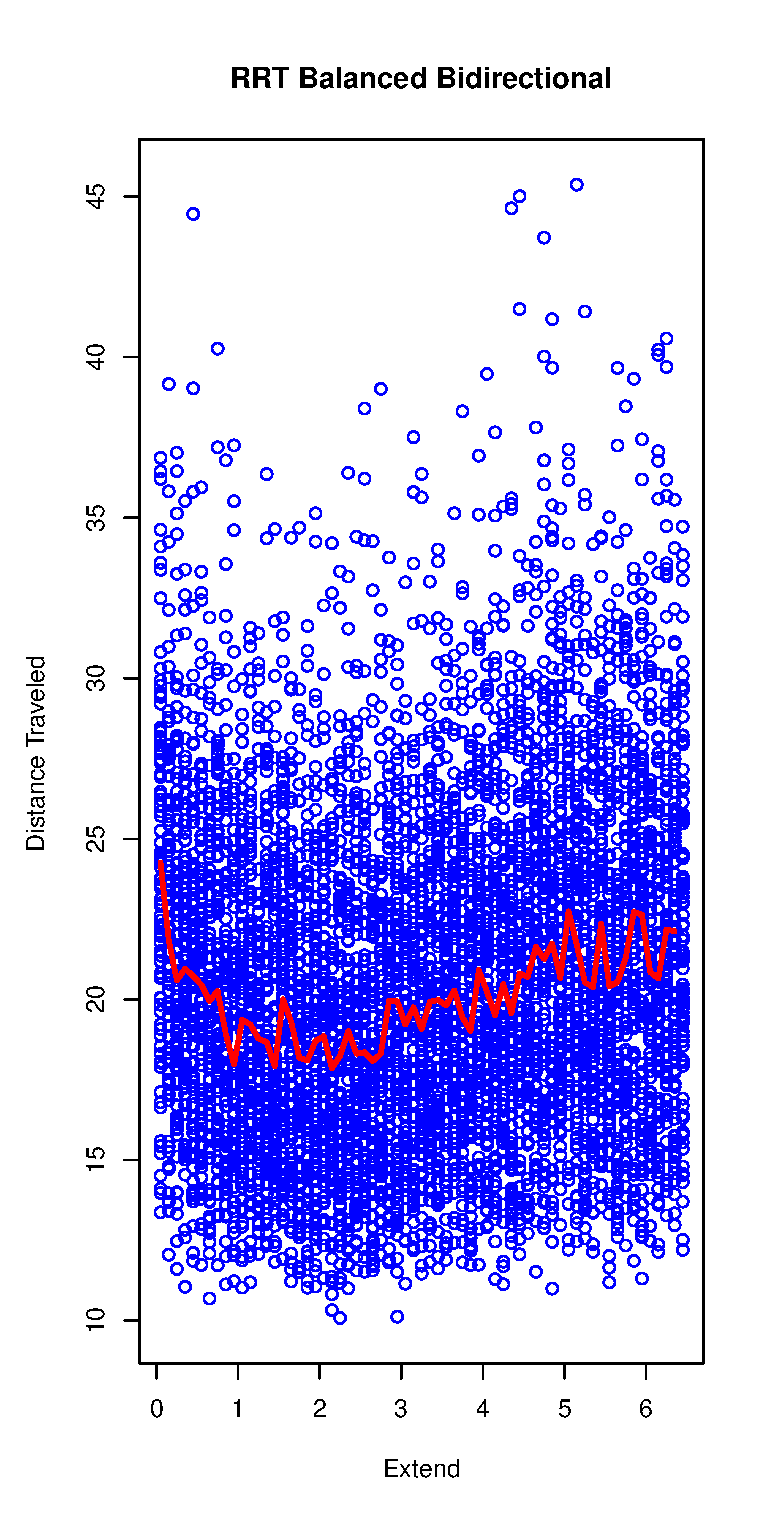
\includegraphics[width=\figsize]{graphics/balanced_correlation}
 \caption{\(d_J\) of the balanced bidirectional RRT planner (blue) with median highlighted (red).}
 \label{fig:balanced_correlated}
\end{figure}


\subsection{Algorithm comparison}
Figure \ref{fig:medians} displays the \(d_J\) medians of both algorithms
together.
The median distance is observed to be generally longer,
including at the optimal \(\epsilon\), with the balanced bidirectional RRT algorithm.
Whether the difference in \(d_J\) is significant, is investigated below.
\begin{figure}[H]
 \centering
 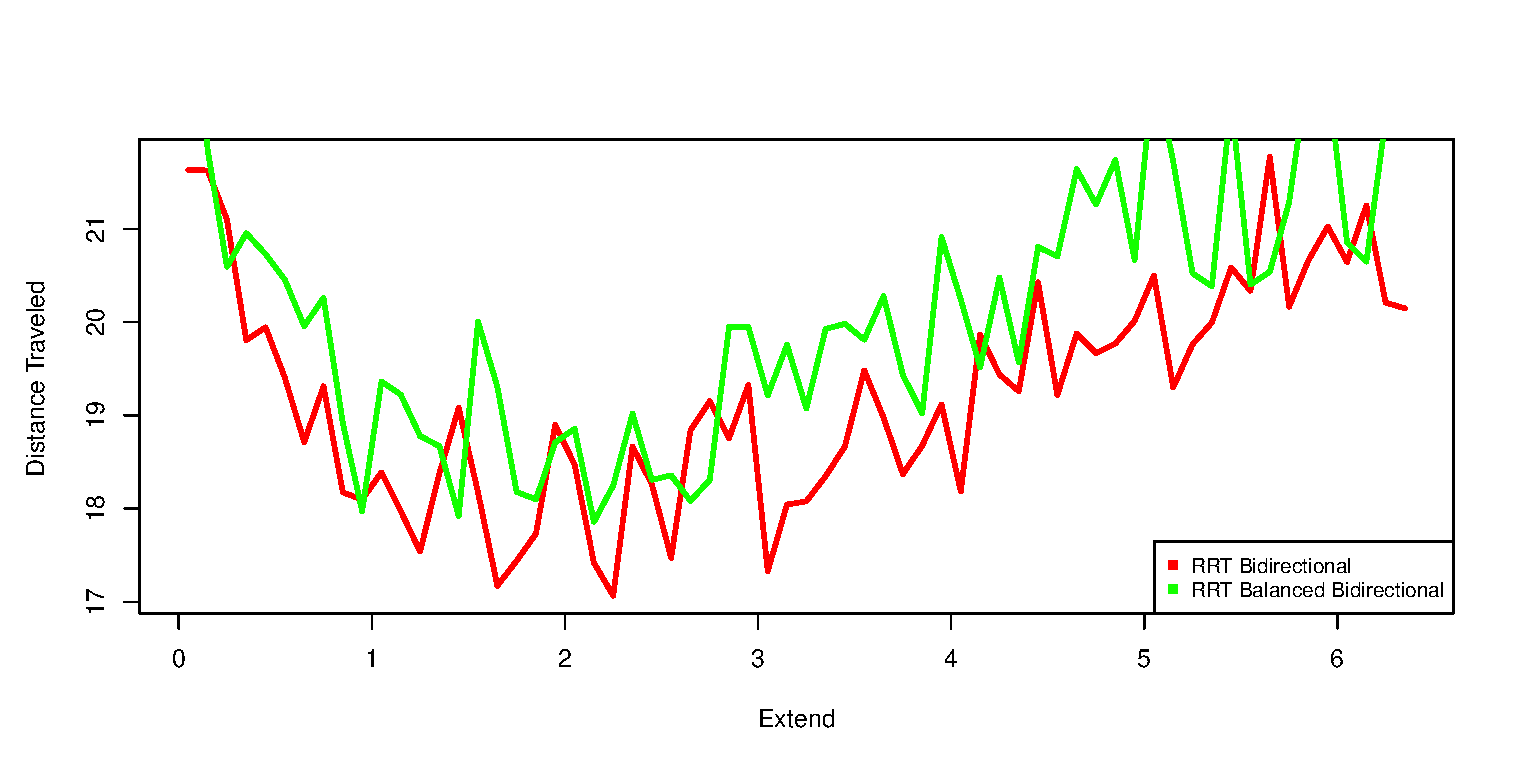
\includegraphics[width=\figsize]{graphics/compare_distance}
 \caption{Medians of \(d_J\) for the RRT planners.}
 \label{fig:medians}
\end{figure}

By plotting the histogram of the path length with the optimal \(\epsilon\),
as seen in figure \ref{fig:bidir_histogram} and \ref{fig:balanced_histogram}, 
it can be seen that \(d_J\) is not normally distributed. 

\begin{figure}[h]
 \centering
 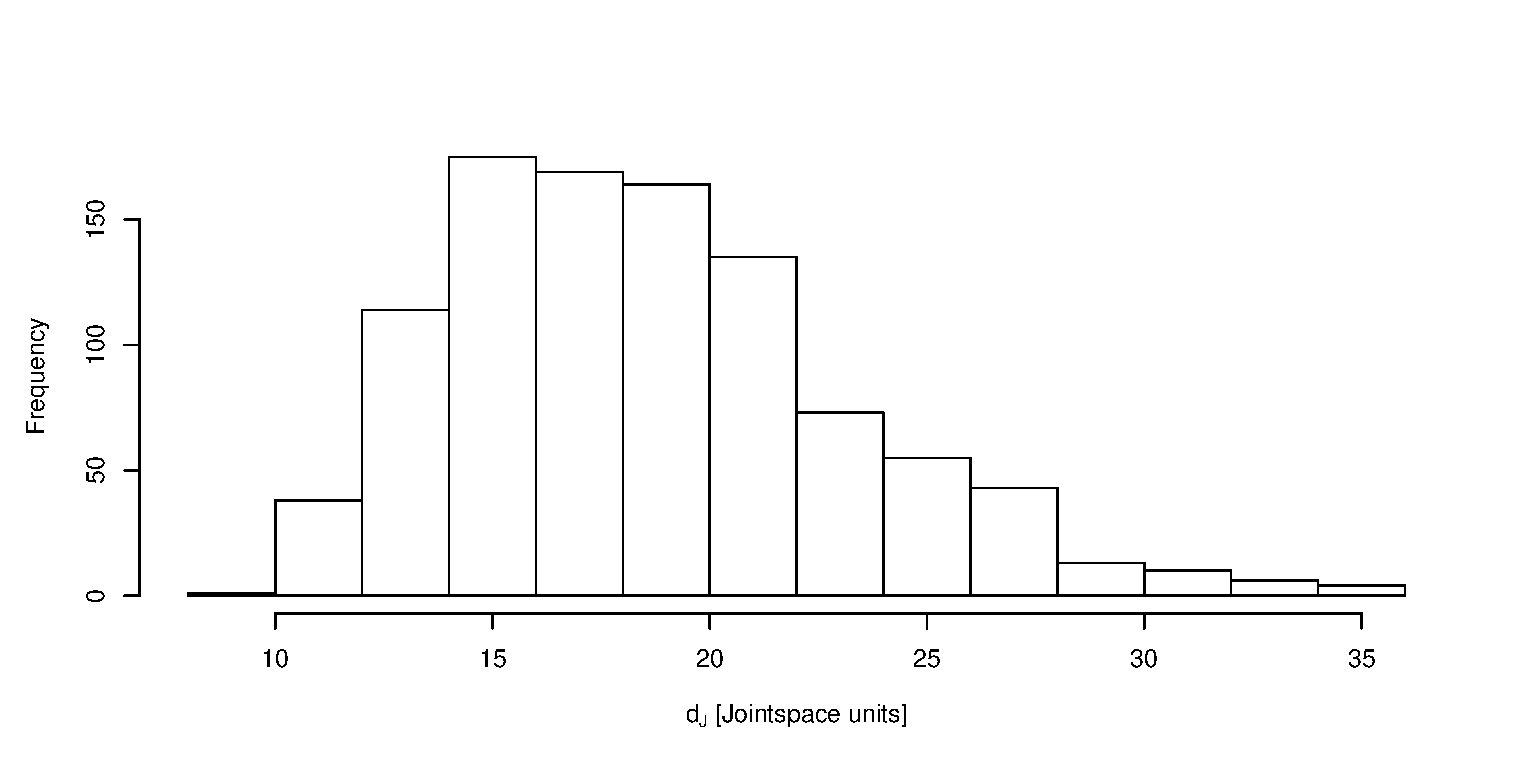
\includegraphics[width=\figsize]{graphics/hist_op_bi}
 \caption{Histogram for \(d_J\) with the optimal \(\epsilon_{bi}\) for the bidirectional RRT planner.}
 \label{fig:bidir_histogram}
\end{figure}

\begin{figure}[h]
 \centering
 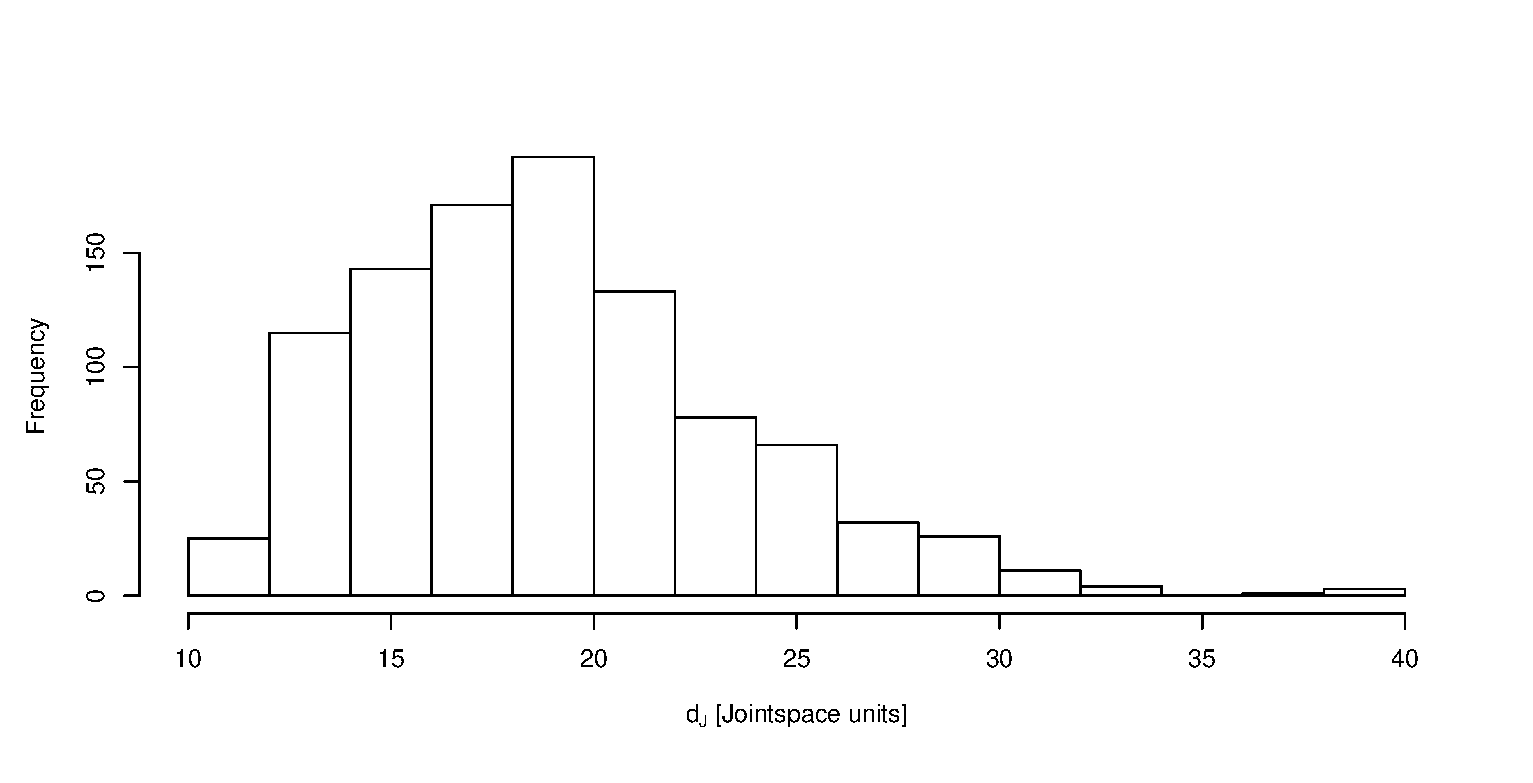
\includegraphics[width=\figsize]{graphics/hist_op_ba}
 \caption{Histogram for \(d_J\) with the optimal \(\epsilon_{ba}\) for the balanced bidirectional RRT planner.}
 \label{fig:balanced_histogram}
\end{figure}

From the QQ plots seen in figures \ref{fig:bidir_qq} and \ref{fig:balanced_qq},
the correlation with a normal distribution is observed to be approximately exponential.

To adjust for this exponentiality, the data is transformed into log space.
The QQ plots of the transformed data,
as seen in figure \ref{fig:bidir_log_qq} and \ref{fig:balanced_log_qq},
imply approximate linearity.
Shapiro Wilks tests are applied to test for normality.
The p-value for the bidirectional RRT is \(4.5\cdot10^{-3}\)
and \(4.2\cdot10^{-4}\) for the balanced bidirectional RRT.
This suggests the data is still not normally distributed.

To test if the variances are equal, an F test is applied.
The p-value is \(0.928\), implying that the variances are significantly different.

Since the variances are different, the method chosen to test if the means are equal,
is Welch's t-test.
The p-value is \(0.042\), implying the means are not significantly different.
Thus, one algorithm can not be said to yield significantly shorter path lengths \(d_J\) than the other
in the given configuration, and \(H_{0,comp}\) is accepted.

\begin{figure}[ht]
 \centering
 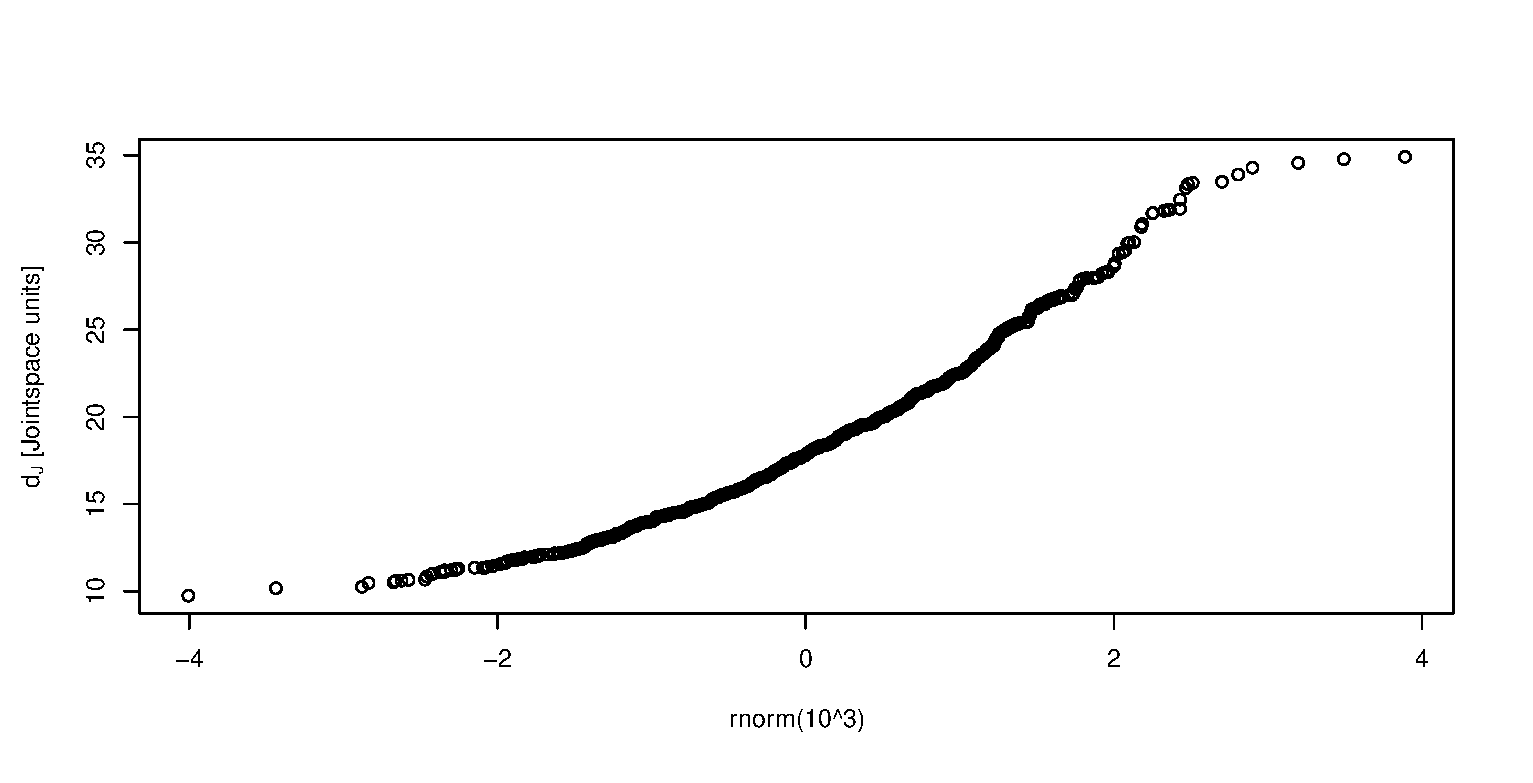
\includegraphics[width=\figsize]{graphics/qq_op_bi}
 \caption{Normal QQ plot for \(d_J\) with the optimal \(\epsilon_{bi}\) for the bidirectional RRT planner.
 The normal distribution is approximated with 1000 samples.}
 \label{fig:bidir_qq}
\end{figure}

\begin{figure}[H]
 \centering
 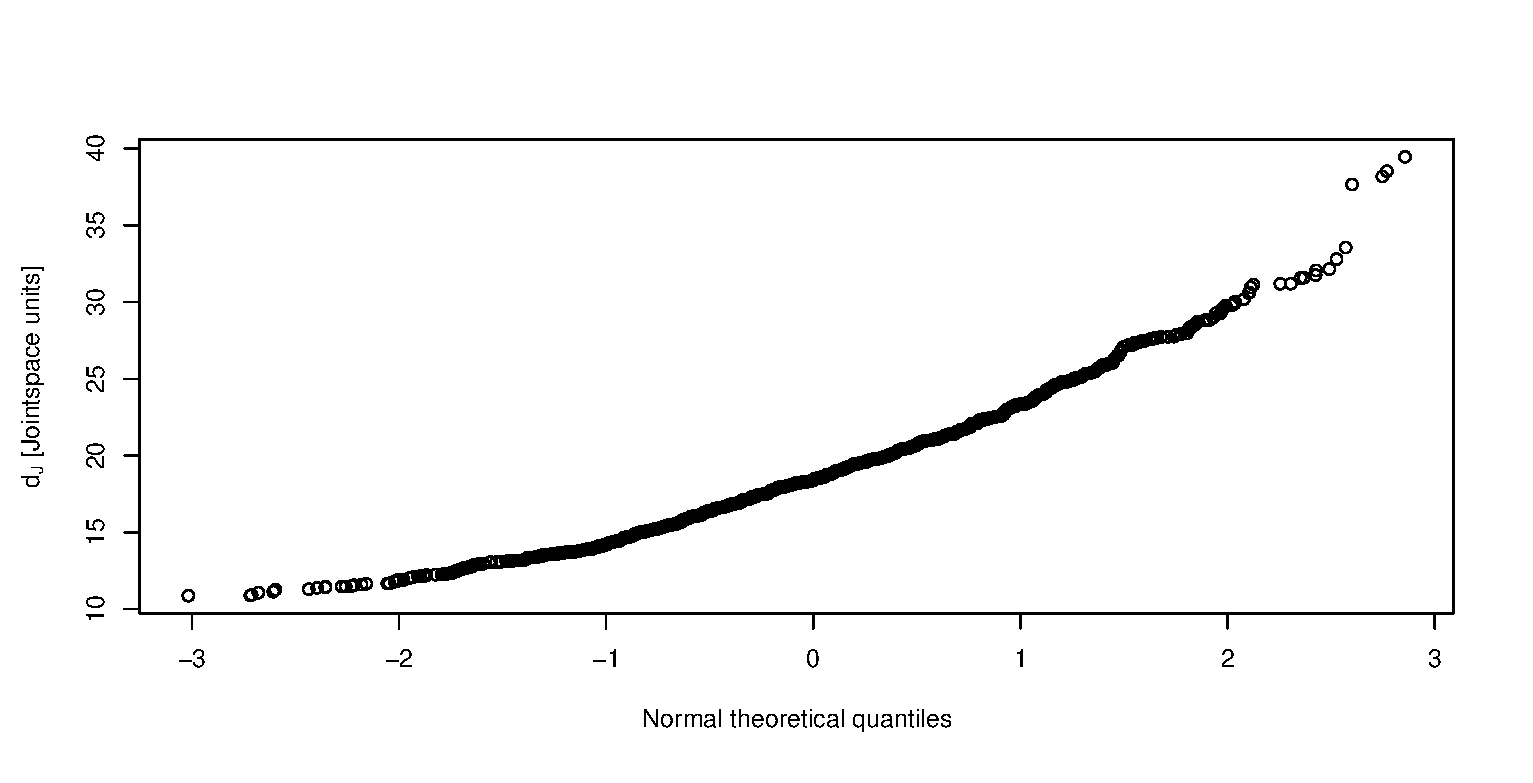
\includegraphics[width=\figsize]{graphics/qq_op_ba}
 \caption{Normal QQ plot for \(d_J\) with the optimal \(\epsilon_{ba}\) for the balanced bidirectional RRT planner.
 The normal distribution is approximated with 1000 samples.}
 \label{fig:balanced_qq}
\end{figure}

\begin{figure}[H]
 \centering
 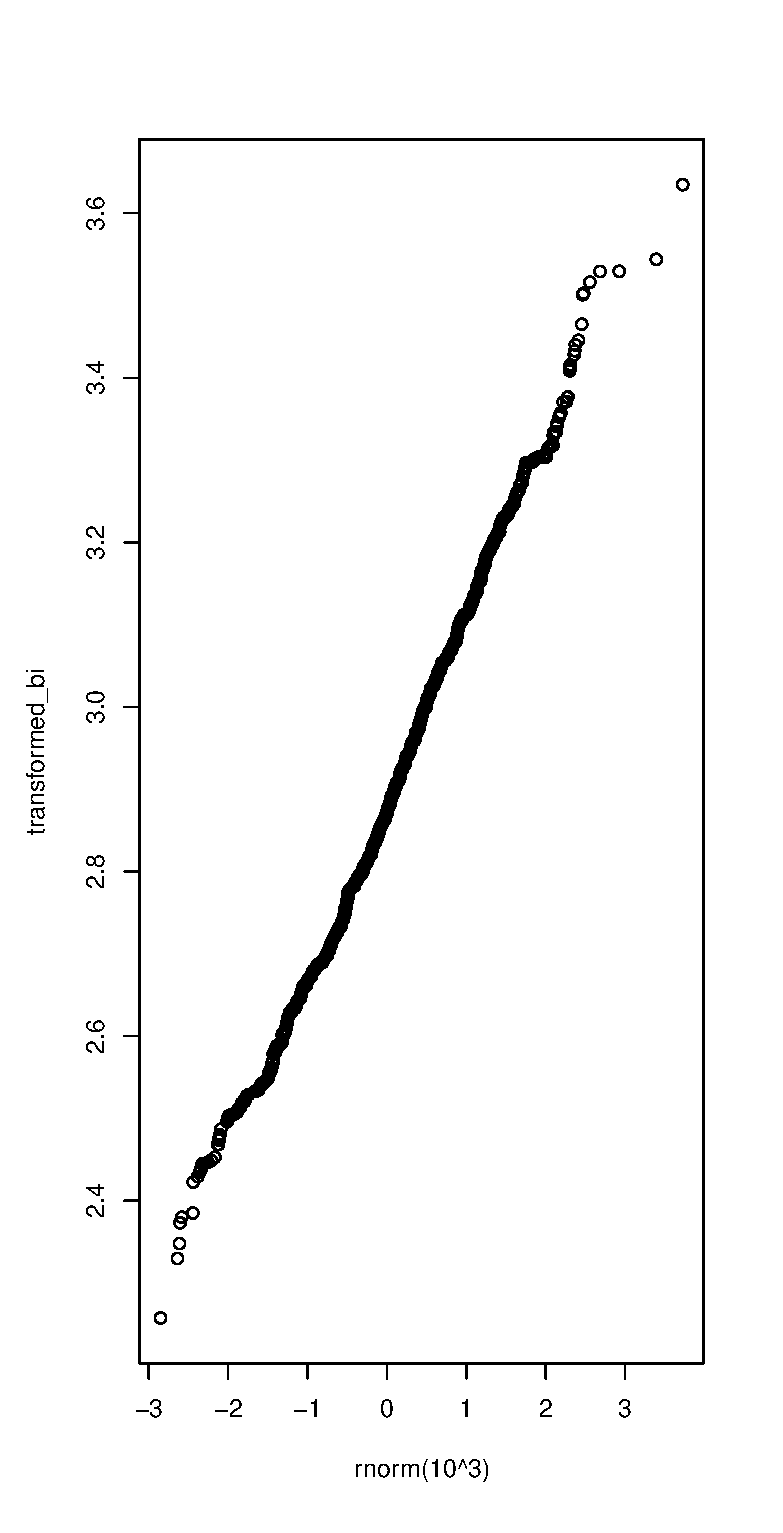
\includegraphics[width=\figsize]{graphics/qq_tran_op_bi}
 \caption{Normal QQ plot for the log transformed \(d_J\) with the optimal \(\epsilon\) for the bidirectional RRT planner. The normal distribution is approximated with 1000 samples.}
 \label{fig:bidir_log_qq}
\end{figure}

\begin{figure}[H]
 \centering
 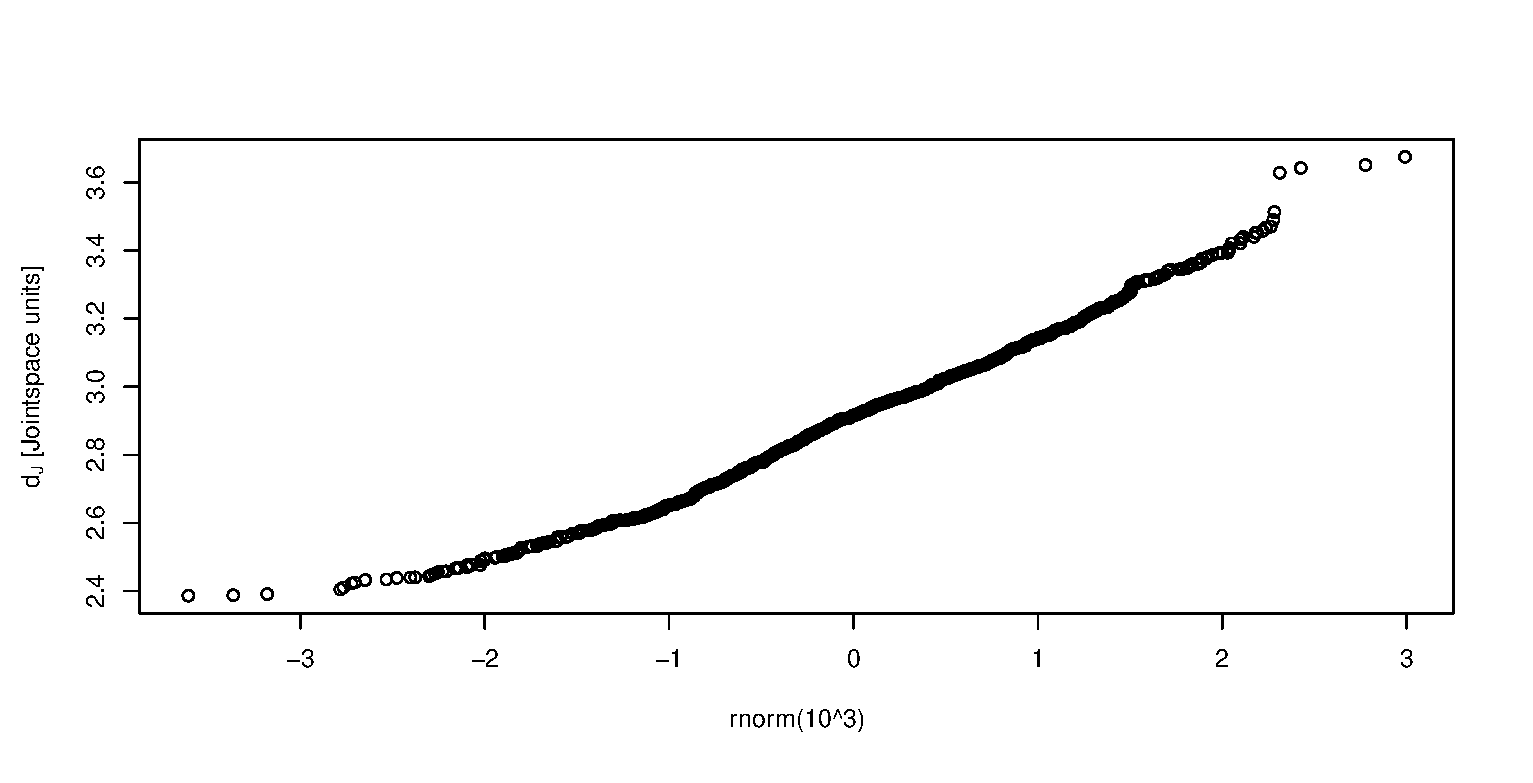
\includegraphics[width=\figsize]{graphics/qq_tran_op_ba}
 \caption{Normal QQ plot for the log transformed \(d_J\) with the optimal \(\epsilon\) for the balanced bidirectional RRT planner. The normal distribution is approximated with 1000 samples.}
 \label{fig:balanced_log_qq}
\end{figure}


